This chapter surveys the work that KickSense builds on. The review is organised from the outside in, beginning with what sports science has established about how goalkeepers actually anticipate penalties, moving through the pose estimation and skeleton based action recognition machinery that makes automated anticipation possible, and closing on the single most directly comparable publication, namely the penalty prediction model of Salazar and Alatrista-Salas \cite{salazar2024}. That paper is the base work for this project and is treated in detail. The chapter ends with two tables, the first summarising the surveyed literature in the conventional comparative format and the second setting KickSense side by side with the base paper across models, datasets, techniques, limitations and future work.

\begin{figure}[H]
    \centering
    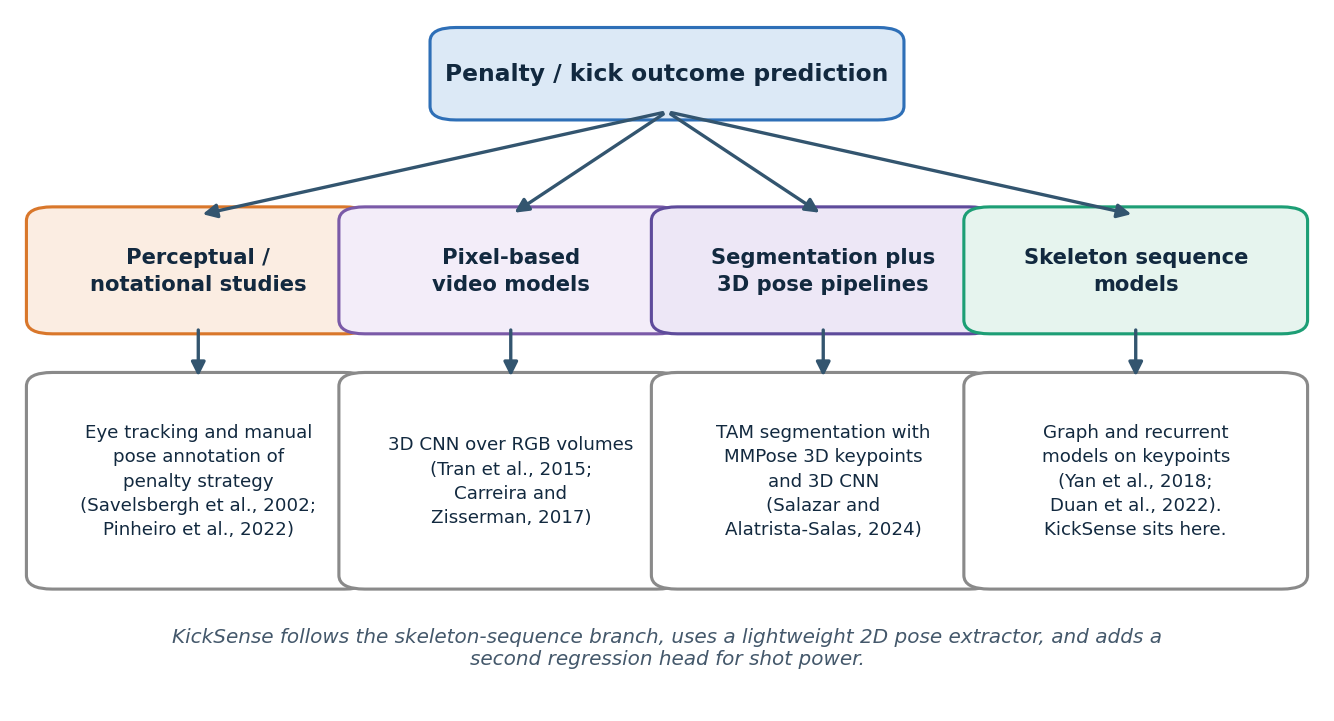
\includegraphics[width=0.98\textwidth]{fig02_research_taxonomy.png}
    \caption{Taxonomy of approaches to penalty and kick outcome prediction}
    \label{fig:taxonomy}
\end{figure}

\noindent
\textbf{Description:} This taxonomy positions KickSense within the existing literature. The leftmost branch covers perceptual and notational studies that established which body cues carry directional information but which rely on human observers. The middle branches cover automated approaches that operate on pixels, either directly through three dimensional convolution or through a segmentation stage followed by three dimensional pose recovery. The rightmost branch covers skeleton sequence models, which is where KickSense sits, using a lightweight two dimensional pose extractor and adding a regression head for shot power that none of the surveyed works provide.

\section{Perceptual Foundations of Penalty Anticipation}

The premise that a penalty kick can be predicted before ball contact is not an assumption of this project but an established experimental finding. Savelsbergh, Williams, van der Kamp and Ward studied expert and novice goalkeepers responding to filmed penalty kicks with a joystick while their eye movements were recorded \cite{savelsbergh2002}. Expert goalkeepers predicted the direction of the kick more accurately, initiated their response later, and made fewer corrective movements, which indicates that they were extracting reliable information from the kicker's body rather than guessing early and adjusting. The eye tracking data localises that information precisely. Novices spent longer fixating the trunk, arms and hips, whereas experts concentrated on the kicking leg, the non kicking leg and the ball region, particularly in the moments immediately before foot to ball contact.

This result is directly load bearing for KickSense in two ways. First, it confirms that the predictive signal exists in the kinematics of the lower body and is available before contact, which is what justifies building a model that consumes only skeletal motion. Second, it identifies which landmarks should matter most, and this expectation is consistent with the finding of the base paper that the legs are the most influential body part for the prediction task \cite{salazar2024}. The limitation of this line of work, from an engineering perspective, is that it measures human perceptual expertise rather than producing an automated system. It tells us the task is solvable and where to look, but it provides no model, no dataset and no reproducible computational pipeline.

Pinheiro, Jin, da Costa and Lames took a step towards automation by integrating body pose estimation with traditional notational analysis to study penalty kick strategy in elite football \cite{pinheiro2022}. Their contribution is methodological: they demonstrate that pose derived measurements can be combined with event annotation to characterise how elite players approach the penalty spot, and they establish that pose estimation output is meaningful at the level of detail required for penalty analysis. The work remains descriptive rather than predictive, in that it quantifies and compares strategies retrospectively without constructing a model that anticipates the direction of an unseen kick, and the analysis pipeline still requires substantial expert involvement rather than running automatically over arbitrary footage.

\section{Human Pose Estimation}

The technical enabler for all automated approaches in this area is human pose estimation, the recovery of anatomical keypoint coordinates from images. The field was reshaped by OpenPose, presented by Cao, Hidalgo, Simon, Wei and Sheikh, which introduced a bottom up architecture using part affinity fields to associate detected body parts into complete skeletons, enabling real time multi person pose estimation for the first time \cite{cao2019}. OpenPose established the practical viability of pose driven video analysis but is computationally demanding, typically requiring a dedicated graphics processor for interactive performance.

Sun, Xiao, Liu and Wang subsequently introduced the High Resolution Network, which maintains high resolution feature representations throughout the network rather than recovering them from low resolution encodings, and which set a new accuracy standard on standard keypoint benchmarks \cite{sun2019}. The accuracy improvement comes with a further increase in computational cost, which places it outside the constraint set of a project intended to run on consumer hardware.

The pose estimator adopted in KickSense is MediaPipe Pose, built on the BlazePose architecture of Bazarevsky and colleagues \cite{bazarevsky2020}, delivered through the MediaPipe perception framework of Lugaresi and colleagues \cite{lugaresi2019}. BlazePose is designed explicitly for on device real time inference and uses a detector followed by a tracker, where the detector localises the person and the tracker regresses thirty three landmarks. The thirty three landmark topology is a deliberate superset of the seventeen keypoint convention used by common benchmarks, adding hands, feet and facial points, and each landmark is returned with a normalised horizontal coordinate, a normalised vertical coordinate, a depth estimate relative to the hip midpoint, and a visibility confidence. The relevant trade off is explicit. MediaPipe is less accurate than the heaviest available estimators and its depth estimate is a relative regression rather than a metric measurement, but it runs at interactive rates on a laptop central processing unit and requires no specialised hardware, which is precisely the property that makes the KickSense deployment target realistic. The limitation observed in practice, and quantified in Chapter 4, is that MediaPipe degrades sharply when the subject is occluded, small in frame or motion blurred, all of which occur routinely in broadcast penalty footage.

\section{Skeleton Based Action Recognition}

Once a video has been reduced to a sequence of skeletons, the classification problem becomes one of temporal sequence modelling over structured coordinates. Two families of approach dominate the literature.

The first family treats the skeleton as a graph. Yan, Xiong and Lin introduced Spatial Temporal Graph Convolutional Networks, which apply graph convolution over the natural connectivity of the human body in the spatial dimension and over time in the temporal dimension \cite{yan2018}. This encodes the anatomical structure of the skeleton directly into the architecture rather than requiring the network to learn it, and it substantially outperformed earlier recurrent baselines on large action recognition benchmarks. Shi, Zhang, Cheng and Lu extended the idea with an adaptive graph whose topology is learned rather than fixed, together with a second stream operating on bone vectors rather than joint positions \cite{shi2019}. Duan, Zhao, Chen, Lin and Dai later revisited the problem and showed that stacking pose heatmaps into a three dimensional volume and applying a three dimensional convolutional network is more robust than graph convolution on joint coordinates, particularly when the pose estimates are noisy \cite{duan2022}.

The second family treats the flattened skeleton as an ordinary multivariate time series and models it with recurrent or convolutional sequence architectures. The Long Short Term Memory unit of Hochreiter and Schmidhuber remains the standard recurrent building block because its gating mechanism allows gradients to propagate over long sequences without vanishing \cite{hochreiter1997}. A common and effective hybrid, and the one adopted by KickSense, places one dimensional convolutions before the recurrent layers so that the convolutions extract short range local motion patterns across neighbouring frames while the recurrent layers integrate those patterns over the whole sequence.

The choice of the recurrent hybrid over the graph based family in this project is driven by dataset size rather than by any claim of superiority. Graph convolutional and heatmap volume approaches were validated on benchmarks containing tens of thousands of labelled sequences. With two hundred and twenty five sequences available, a model with a quarter of a million parameters already overfits, and the additional capacity of a graph network would make that worse rather than better. Evaluating a spatial temporal graph network on this task once the corpus is substantially larger is therefore listed in the future work of Chapter 5.

\section{Video Level Action Recognition}

For completeness it is worth recording the pixel based alternative, since the base paper follows it. Tran, Bourdev, Fergus, Torresani and Paluri demonstrated that three dimensional convolutional networks learn effective spatiotemporal features directly from raw video volumes \cite{tran2015}. Simonyan and Zisserman proposed a two stream design in which one branch consumes appearance and a second consumes optical flow, showing that explicit motion representation is valuable \cite{simonyan2014}. Carreira and Zisserman then introduced the Inflated three dimensional network, which converts a strong two dimensional image classifier into a three dimensional video model by inflating its filters and initialising them from image pretrained weights, which remains a standard baseline for video classification \cite{carreira2017}. Wang and colleagues addressed the sampling problem with Temporal Segment Networks, which sample sparsely across the whole clip rather than densely over a short window \cite{wang2016}.

The strength of this family is that it discards nothing, since colour, texture, ball position and context all remain available to the network. The weaknesses matter a great deal at the scale of a final year project. These models contain tens of millions of parameters, require large pretraining corpora to be effective, and consume video volumes of hundreds of thousands of values per frame, all of which is difficult to justify when the labelled dataset contains a few hundred clips. They are also sensitive to nuisance variation such as camera angle, stadium, kit colour and lighting, none of which carries information about shot direction, and with a small dataset a high capacity pixel model will readily latch onto exactly those spurious correlations.

\section{Football Specific Datasets and Tooling}

The absence of a suitable public dataset is a defining constraint of this project, so it is worth being specific about what does exist. Giancola, Amine, Dghaily and Ghanem released SoccerNet, a large scale dataset for action spotting in broadcast football video, later substantially extended by Deliège and colleagues as SoccerNet version two with a far richer action vocabulary and additional tasks \cite{giancola2018,deliege2021}. These resources are valuable and widely used, but their annotation granularity is the event level, marking that a penalty occurred at a given timestamp, and they do not annotate the direction the penalty was aimed towards or the power with which it was struck. Pappalardo and colleagues published a large public collection of spatiotemporal match event data covering multiple competitions, which is again event level and contains no video or pose information \cite{pappalardo2019}.

The consequence is unavoidable. A model that predicts penalty direction from body motion requires per clip direction labels, and no public dataset provides them. Both the base paper and this project therefore had to construct a bespoke corpus, and since neither corpus is the same as the other, any numerical comparison between them measures the difficulty of two different datasets as much as it measures the quality of two different models. This point governs the way results are compared in Chapter 4.

On the tooling side, the base paper relies on Track Anything for its segmentation stage, an interactive video object segmentation and tracking system built on the Segment Anything foundation model \cite{yang2023,kirillov2023}, and on MMPose for three dimensional pose recovery \cite{mmpose2020}. KickSense is implemented with TensorFlow and Keras for modelling \cite{abadi2016} and scikit-learn for splitting, class weighting and metric computation \cite{pedregosa2011}, with optimisation by Adam \cite{kingma2015} and regularisation by dropout and batch normalisation \cite{srivastava2014,ioffe2015}.

\section{The Base Paper in Detail}

Salazar and Alatrista-Salas present the work most directly comparable to KickSense, published at the ninth International Conference on Machine Learning Technologies in Oslo in 2024 \cite{salazar2024}. Their objective is the same as ours, namely to predict the region of the goal towards which a penalty will be directed from the pose of the kicker, and their framing of the problem as a three way regional classification is the framing this project adopted.

Their methodology proceeds in three stages. They first construct a corpus of penalty kick videos, since no public equivalent exists. They then combine semantic video segmentation using Track Anything with three dimensional pose estimation using MMPose, the purpose of the segmentation stage being to isolate the kicker from the background and from other players so that the pose estimator operates on a clean subject. They finally compare three deep learning models for the prediction task and conduct an analysis of which part of the player's body most affects the prediction, concluding that the legs are the most influential region.

The strengths of the approach are real. The segmentation stage directly attacks the occlusion and clutter problem that degrades pose estimation on broadcast footage, and it does so more thoroughly than a quality filter can, because it improves the input rather than discarding bad cases. Three dimensional pose recovery captures depth relationships, in particular the rotation of the pelvis away from the image plane, that a two dimensional projection can only represent indirectly. Comparing three model families rather than presenting one is methodologically sound, and the body part influence study is exactly the kind of interpretability analysis that makes a result useful to a coach rather than merely accurate.

The limitations are equally real and shaped the design of this project. The pipeline is heavy, since interactive segmentation followed by three dimensional pose estimation followed by three dimensional convolution is far beyond what runs on a phone or on a laptop without a graphics processor, which forecloses the grassroots deployment that motivates KickSense. The corpus is bespoke and not publicly released, so the reported accuracy cannot be independently reproduced and cannot serve as a benchmark. The prediction is restricted to the goal region and does not include any estimate of shot power, so a goalkeeper receives no information about how firmly the ball will be struck. The segmentation stage as described requires human interaction to specify the object to be tracked, which limits the degree to which the pipeline can be applied automatically at scale.

KickSense responds to each of these limitations with a specific design decision rather than a general aspiration. In place of segmentation followed by three dimensional pose estimation, it applies a lightweight two dimensional pose estimator with an explicit quality gate, which removes the human in the loop and reduces the computational cost by orders of magnitude at the price of a measured rejection rate. In place of a single classification head it uses a multi task head that predicts direction and power from a shared representation. In place of an unpublished corpus it maintains a fully documented annotation file, per clip intermediate artefacts and a fixed stratified split, so that every number in this report can be regenerated from the repository. What KickSense does not claim is superiority, since the datasets differ and the comparison would be meaningless, and this is stated explicitly in the summary table and revisited in Chapter 4.

\section{Comparison of Surveyed Literature}

\renewcommand{\arraystretch}{1.3}
\setlength{\tabcolsep}{4pt}
\small

\begin{longtable}{|c|c|>{\raggedright\arraybackslash}p{2.5cm}|
>{\raggedright\arraybackslash}p{2.9cm}|
>{\raggedright\arraybackslash}p{3.0cm}|
>{\raggedright\arraybackslash}p{3.0cm}|}

\hline
\textbf{Ref} & \textbf{Year} & \textbf{Author(s)} &
\textbf{Approach} & \textbf{Contribution} & \textbf{Limitation} \\
\hline
\endfirsthead

\hline
\textbf{Ref} & \textbf{Year} & \textbf{Author(s)} &
\textbf{Approach} & \textbf{Contribution} & \textbf{Limitation} \\
\hline
\endhead

\hline
\multicolumn{6}{r}{\textit{Continued on next page}} \\
\hline
\endfoot

\hline
\endlastfoot

\cite{savelsbergh2002} & 2002 & Savelsbergh et al. &
Eye tracking of expert and novice goalkeepers responding to filmed penalties &
Proves directional information is available before contact and localises it to the kicking and non kicking leg &
Measures human perception only; provides no automated model, dataset or pipeline \\ \hline

\cite{pinheiro2022} & 2022 & Pinheiro et al. &
Body pose estimation combined with notational analysis of elite penalties &
Shows pose measurements are meaningful at the granularity penalty analysis requires &
Descriptive rather than predictive; needs substantial expert involvement per clip \\ \hline

\cite{cao2019} & 2019 & Cao et al. &
Bottom up multi person pose estimation using part affinity fields (OpenPose) &
Made real time multi person pose estimation practical and widely reusable &
Computationally heavy; typically needs a dedicated graphics processor \\ \hline

\cite{sun2019} & 2019 & Sun et al. &
High resolution representation learning for keypoint detection (HRNet) &
Set a new accuracy standard on standard keypoint benchmarks &
Cost rises further; unsuited to on device or laptop only deployment \\ \hline

\cite{bazarevsky2020} & 2020 & Bazarevsky et al. &
Detector plus tracker regression of 33 landmarks for on device use (BlazePose) &
Interactive rate pose estimation on commodity hardware, adopted by this project &
Lower accuracy than heavy estimators; depth is relative, and it fails under occlusion \\ \hline

\cite{yan2018} & 2018 & Yan et al. &
Spatial temporal graph convolution over skeleton joints (ST-GCN) &
Encodes body connectivity into the architecture and beat recurrent baselines &
Validated on tens of thousands of sequences; overfits small corpora \\ \hline

\cite{shi2019} & 2019 & Shi et al. &
Adaptive graph topology with an additional bone vector stream &
Learned topology and second stream improve skeleton action accuracy &
Higher capacity and more hyperparameters, worsening small data overfitting \\ \hline

\cite{duan2022} & 2022 & Duan et al. &
Stacked pose heatmap volumes processed by a 3D CNN (PoseC3D) &
More robust than joint coordinate graphs when pose estimates are noisy &
Reintroduces the memory and compute cost of 3D convolution \\ \hline

\cite{tran2015} & 2015 & Tran et al. &
3D convolution learned directly on raw RGB video volumes (C3D) &
Established spatiotemporal feature learning from pixels &
Tens of millions of parameters; needs large pretraining corpora \\ \hline

\cite{simonyan2014} & 2014 & Simonyan and Zisserman &
Two stream network combining appearance and optical flow &
Showed explicit motion representation materially improves accuracy &
Optical flow computation is expensive and adds a preprocessing dependency \\ \hline

\cite{carreira2017} & 2017 & Carreira and Zisserman &
Filters of a 2D image classifier inflated into 3D (I3D) &
Strong transferable video baseline through image pretraining &
Large model; sensitive to nuisance variation such as camera angle and kit \\ \hline

\cite{hochreiter1997} & 1997 & Hochreiter and Schmidhuber &
Gated recurrent unit for long range sequence modelling (LSTM) &
Enables gradient flow over long sequences, the backbone used here &
Sequential computation limits parallelism relative to newer architectures \\ \hline

\cite{giancola2018} & 2018 & Giancola et al. &
Large scale action spotting dataset for broadcast football (SoccerNet) &
Provides scale and a standard protocol for football video research &
Event level labels only; no penalty direction, power or pose annotation \\ \hline

\cite{deliege2021} & 2021 & Deliège et al. &
Extended action vocabulary and additional tasks (SoccerNet-v2) &
Richer annotation and more football video tasks &
Still event level; cannot supervise direction prediction \\ \hline

\cite{pappalardo2019} & 2019 & Pappalardo et al. &
Public spatiotemporal match event dataset across competitions &
Large reusable public football event resource &
No video and no pose data, so unusable for this task \\ \hline

\cite{yang2023} & 2023 & Yang et al. &
Interactive video object segmentation and tracking (Track Anything) &
High quality subject isolation in video, used by the base paper &
Requires human interaction to initialise the tracked object \\ \hline

\cite{salazar2024} & 2024 & Salazar and Alatrista-Salas &
TAM segmentation with MMPose 3D pose, three deep models compared, body part influence study &
Closest prior work; identifies the legs as the most influential region &
Heavy pipeline, unpublished corpus, no power estimate, human in the loop segmentation \\ \hline

\caption{Summary of the surveyed literature on pose estimation, skeleton action recognition and penalty prediction}
\label{tab:literature-summary}
\end{longtable}
\normalsize
\clearpage

\section{Comparison of KickSense with the Base Paper}

Table \ref{tab:basepaper-compare} sets the base paper and KickSense against each other across the dimensions that matter for this project. The final row is the most important one, because it states what each work leaves undone and therefore what the remaining phase of this project is committed to delivering.

\renewcommand{\arraystretch}{1.35}
\setlength{\tabcolsep}{5pt}
\small

\begin{longtable}{|>{\raggedright\arraybackslash\bfseries}p{2.6cm}|
>{\raggedright\arraybackslash}p{5.6cm}|
>{\raggedright\arraybackslash}p{5.6cm}|}

\hline
\textbf{Dimension} & \textbf{Salazar and Alatrista-Salas (2024)} & \textbf{KickSense (this project)} \\
\hline
\endfirsthead

\hline
\textbf{Dimension} & \textbf{Salazar and Alatrista-Salas (2024)} & \textbf{KickSense (this project)} \\
\hline
\endhead

\hline
\multicolumn{3}{r}{\textit{Continued on next page}} \\
\hline
\endfoot

\hline
\endlastfoot

The work &
Football Penalty Kick Prediction Model Based on Kicker's Pose Estimation, ICMLT 2024, pages 196 to 203, ACM &
KickSense: Intelligent Penalty Kick Analysis Using Pose Estimation, Bahria University final year project \\ \hline

Publication year &
2024 &
2026 (in progress) \\ \hline

Prediction target &
Goal region towards which the kick will land, three classes &
Shot direction in three classes (Left, Center, Right) plus a shot power score from one to ten \\ \hline

Models used &
Three deep learning models compared, applied to 3D pose sequences derived from segmented video &
Multi task CNN-LSTM with a shared encoder, a softmax direction head and a sigmoid power head, 249,220 parameters \\ \hline

Pose representation &
3D pose estimated with MMPose after semantic video segmentation with Track Anything &
2D pose with relative depth and visibility from MediaPipe Pose at model complexity two, 33 landmarks per frame \\ \hline

Dataset used &
Bespoke corpus of penalty kick videos constructed by the authors and not publicly released &
Bespoke corpus of 301 collected clips, 259 fully annotated, 225 usable after pose quality filtering, split 157 / 34 / 34 \\ \hline

Reason the datasets differ &
No public penalty direction dataset exists, so the authors had to build their own; the corpus is not distributed &
For the same reason a new corpus had to be built, and because the base corpus is unavailable it could not be reused. The two datasets therefore differ in size, camera angles, competitions and annotation schema \\ \hline

Techniques in common &
Pose estimation as the feature source, deep learning over temporal pose sequences, three way regional classification, analysis of which body part drives the prediction &
Pose estimation as the feature source, deep learning over temporal pose sequences, three way directional classification, and the same expectation that lower body landmarks dominate \\ \hline

Techniques that differ &
Semantic video segmentation before pose estimation, 3D pose recovery, comparison of three model families &
Hip centred normalisation and torso height scaling, fixed 26 step temporal resampling, explicit pose quality gate, fivefold augmentation with left to right mirroring, multi task loss with a weighted power term, ablation study over architecture and training choices \\ \hline

Evaluation &
Accuracy of regional prediction with a study of body part influence &
Accuracy, weighted and per class precision, recall and F1, confusion matrix for direction; MAE, MSE and RMSE for power; all reported against a stated 33.3 percent random baseline on a held out test split \\ \hline

Limitations &
Heavy pipeline unsuitable for on device use, corpus not released so results are not reproducible, no shot power output, segmentation requires human initialisation &
Small dataset of 225 sequences, unbalanced classes with only 58 centre examples, subjective power annotation, ball placement label collected but unused, accuracy above chance but not yet competition ready \\ \hline

Basis of comparison &
Reports accuracy on its own private corpus &
Reports accuracy on its own corpus. Because neither corpus is available to the other, no head to head accuracy claim is made in this report. Only methodology, cost and output scope are compared \\ \hline

Future work &
Indicated directions include extending the corpus and refining the body part influence analysis &
Replace the subjective power scale with a measurement derived from frame to frame ball displacement; integrate the existing ball placement annotation as an auxiliary task; run a systematic hyperparameter search over learning rate, sequence length, dropout and loss weighting; resolve the remaining pose configuration mismatch between the training and inference paths; expand the corpus with further recorded sessions; evaluate a spatial temporal graph network once the corpus supports it; and deliver the Flutter web and Android client on top of the existing FastAPI service \\ \hline

\caption{Comparison of the base paper and KickSense across models, datasets, techniques, limitations and future work}
\label{tab:basepaper-compare}
\end{longtable}
\normalsize

\section{Summary of the Literature Review}

Three conclusions follow from this review and carry directly into the methodology of Chapter 3. First, the task is legitimate, because controlled perceptual experiments establish that directional information is present in the kicker's body motion before ball contact and is concentrated in the legs \cite{savelsbergh2002}. Second, the appropriate feature representation for a project constrained to consumer hardware is the skeleton rather than the pixel volume, since it reduces each frame by three orders of magnitude, removes nuisance variation that a small dataset would otherwise be exploited by, and is recoverable in real time by a lightweight estimator \cite{bazarevsky2020}. Third, no public dataset can supervise this task, so a bespoke annotated corpus is a prerequisite rather than an optional contribution, and the absence of a shared benchmark means the honest form of comparison against prior work is methodological rather than numerical.

\clearpage
